%&tex
\chapter{Experiments}
%
\begin{table}
	\caption{Difficulties of datasets: articulation, intra-class variance, background clutter and viewpoint variation}
	\label{tab:challenges}
	\begin{tabular}{l|rrrr}
		Dataset &  Articul.& Var. &  Backgr.& Viewp.  \\ \hline
		CelebA &   &  &  &    \\
		Cat Head & &  \checkmark&  &   \\
		CUB-200-2011 & & \checkmark& \checkmark&   \\
		Human3.6M &\checkmark& &  & \checkmark  \\
		BBC Pose &  \checkmark&  & \checkmark&  \\
		Dogs Run & \checkmark& \checkmark& \checkmark&   \\
		Penn Action & \checkmark& \checkmark& \checkmark& \checkmark\\
	\end{tabular}
\end{table}
%
% SHOW DISENTANGLING: SHAPE
\begin{figure}[t]
	\begin{subfigure}{0.5\textwidth}
	\centering
	\includegraphics[trim={0cm 0cm 0cm 0cm},clip, width=1.\linewidth]{fig/shape6white}\caption{}
	\label{fig:shape_penn}
	\end{subfigure}
	\begin{subfigure}{0.5\textwidth}
	\centering
	\includegraphics[trim={0cm 0cm 0cm 0cm},clip, width=1.\linewidth]{fig/shape_tennis}\caption{}
	\label{fig:shape_tennis}
	\end{subfigure}
	%\begin{subfigure}{0.5\textwidth}
	%\centering
	%\includegraphics[trim={0cm 0cm 0cm 0cm},clip, width=1.\linewidth]{mat/shape_yoga}\caption{}
	%\label{fig:shape_yoga}
	%\end{subfigure}
	\caption{Learned shape representation on Penn Action. For visualization, 13 of 16 part activation maps are plotted in one image. (a) Different instances, showing intra-class consistency and (b) video sequence, showing consistency and smoothness under motion, although each frame is processed individually.}
	\label{fig:shape}
\end{figure}

\section{Shape Learning}
	% SHOW DISCOVERY
	\begin{figure}[htp]
		\centering
		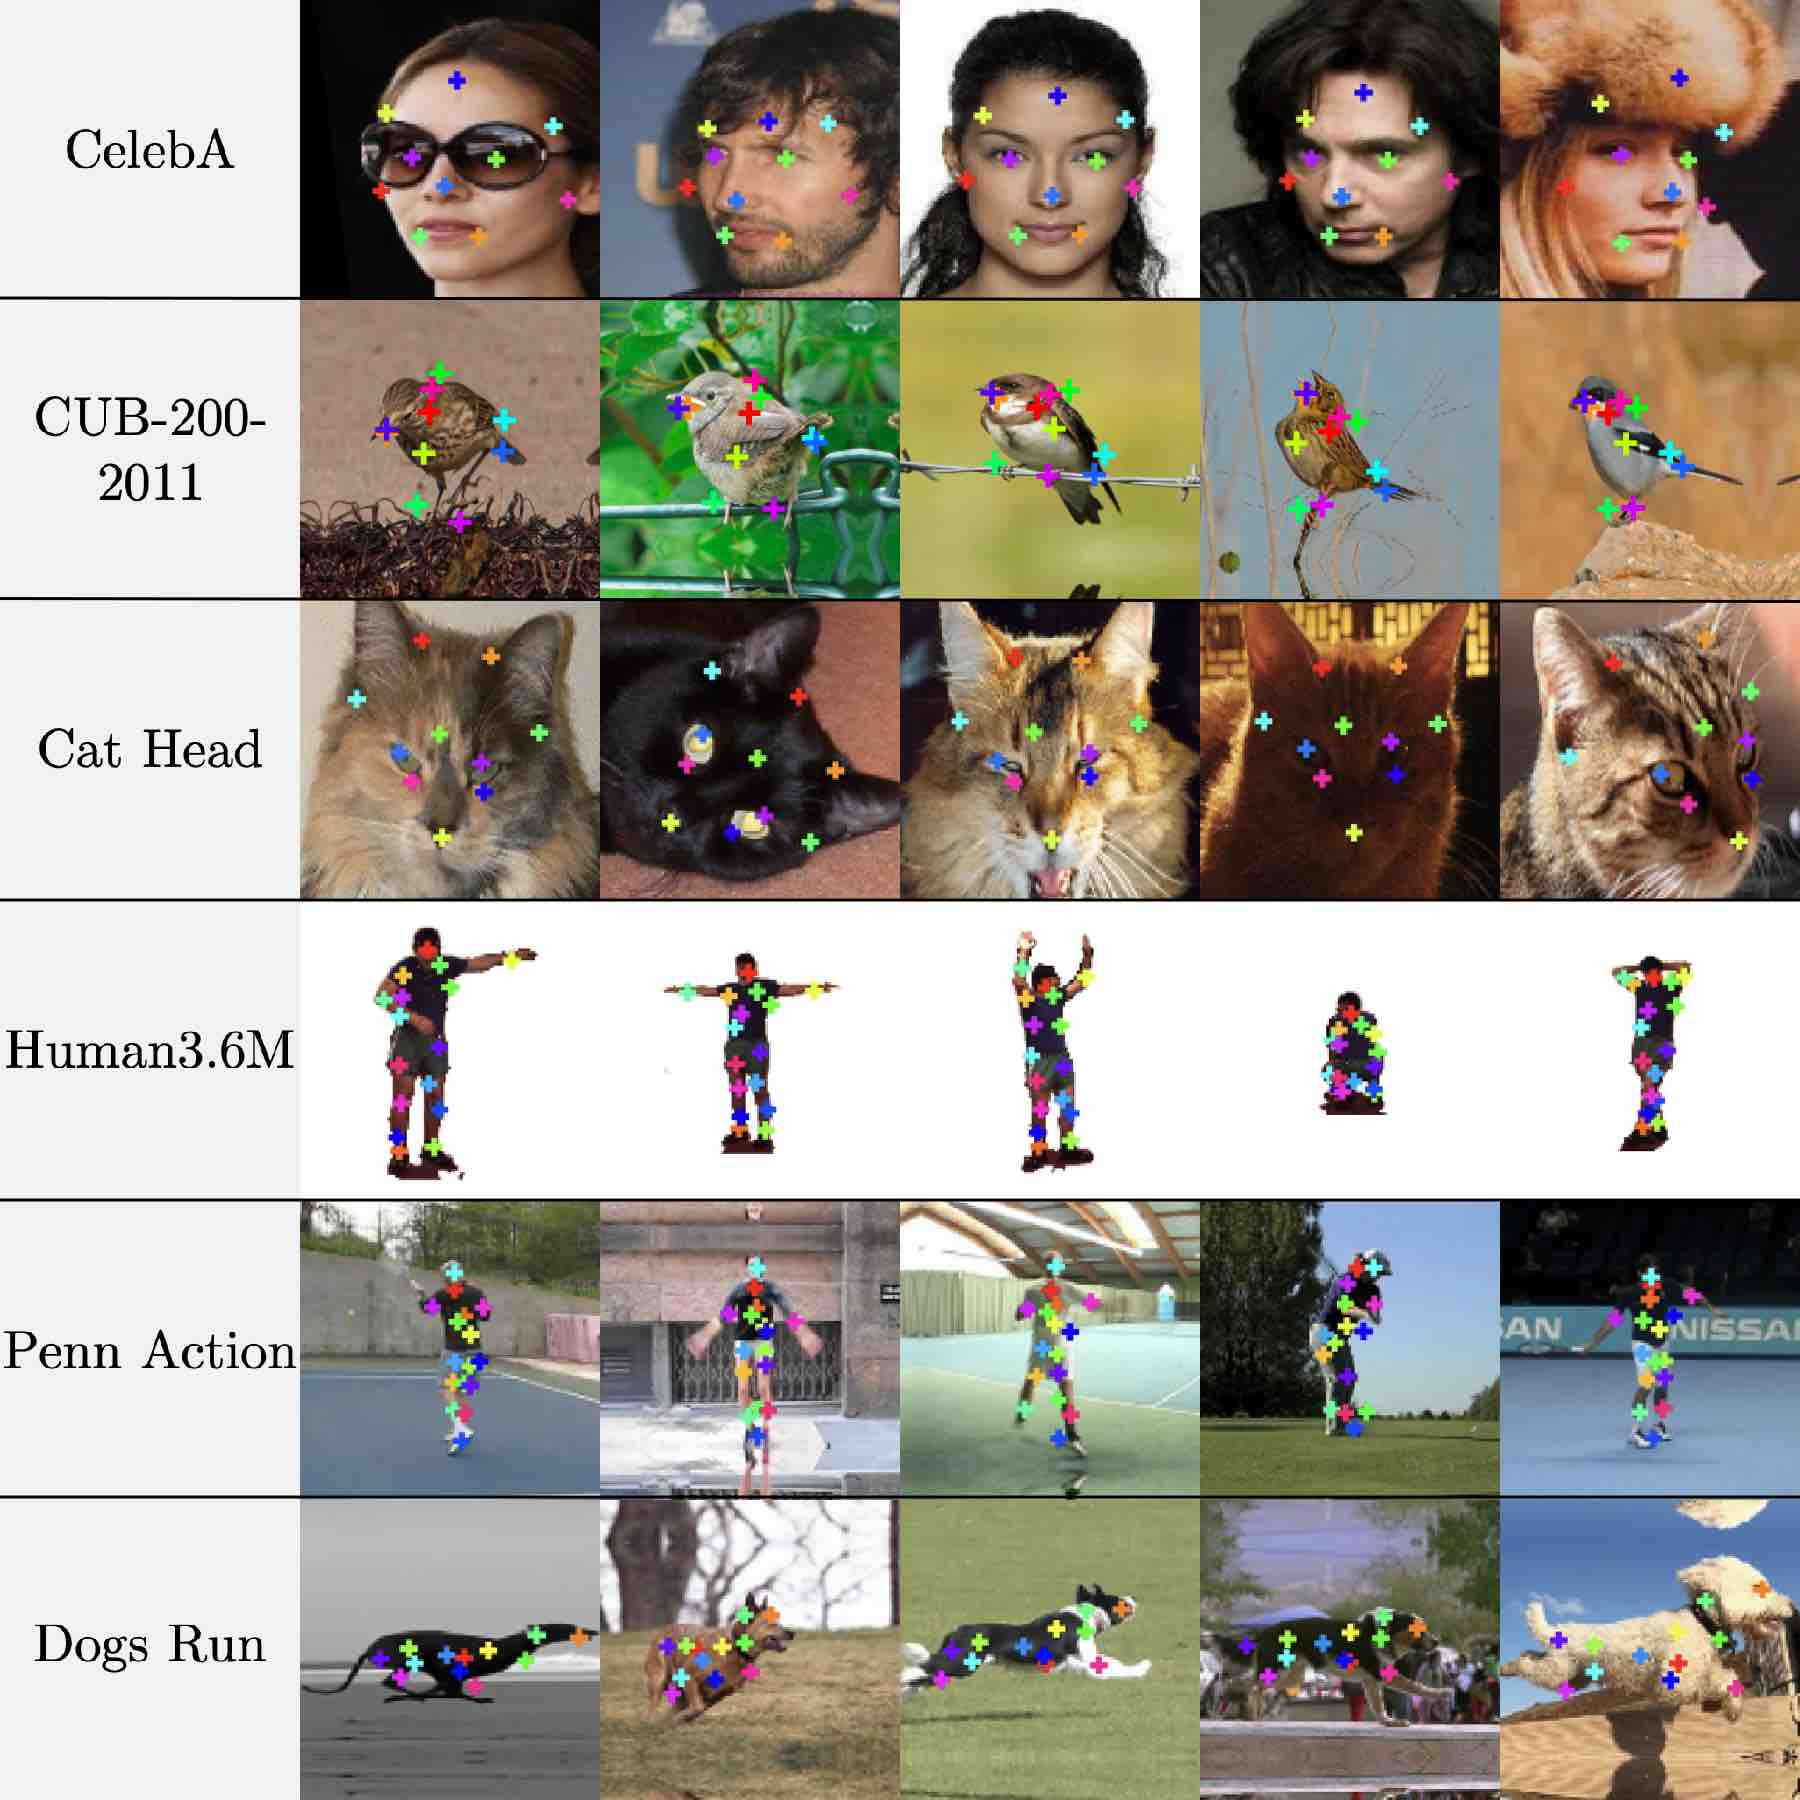
\includegraphics[trim={0cm 0cm 0cm 0cm},clip, width=1.\linewidth]{fig/kp_mania}
		\caption{{Unsupervised discovery of landmarks on diverse object classes such as human or cat faces and birds and for highly articulated human bodies and running dogs.}}
		%(from CelebA, CUB-200-2011 and Cat Head)
		% and on articulated objects such as human bodies and running dogs.}}
		%(from Human3.6M (no background),  Penn Action (real world conditions) and Dogs Run).}}
		\label{fig:kp_mania}
	\end{figure}
	\begin{figure}[htp]
		\centering
		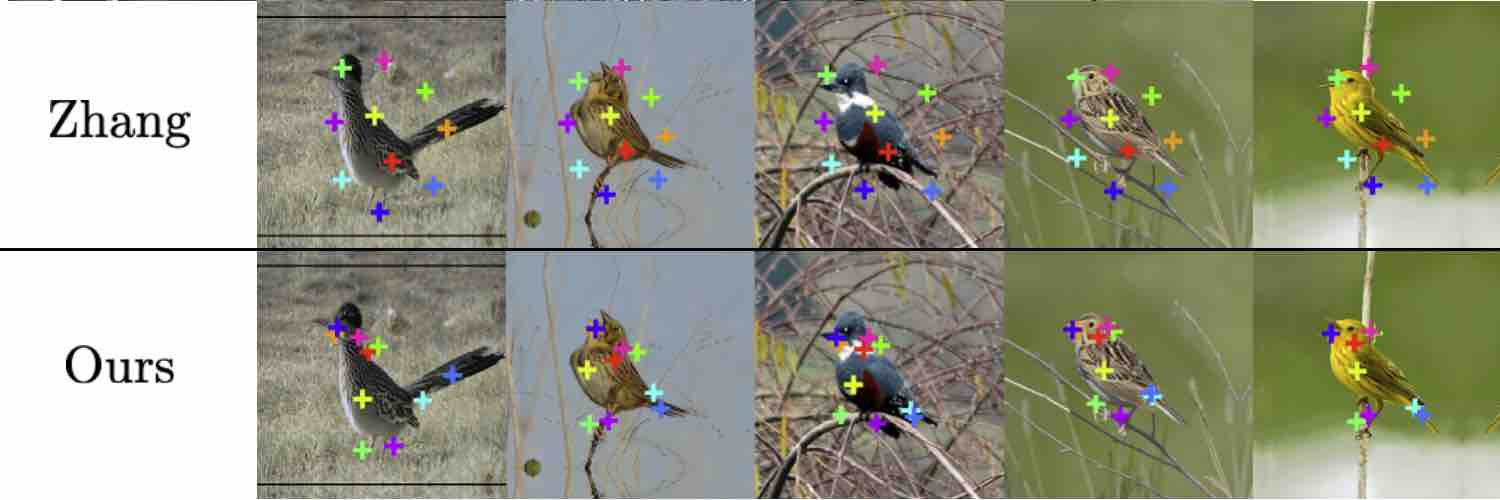
\includegraphics[trim={0cm 0cm 0cm 0cm},clip, width=1.\linewidth]{fig/birds1x3}
		\caption{Comparing discovered keypoints against \cite{zhang18} on CUB-200-2011. We improve on object coverage and landmark consistency. Note our flexible part placement compared to a rather rigid placement of \cite{zhang18} due to their part separation bias.}
		\label{fig:compare}
	\end{figure}
	% STATIC DATASETS: CELEBA, CATS, BIRDS
	% \begin{table}[t]
		% \caption{{Comparison with other unsupervised methods for annotated landmark prediction on the Cat Head, MAFL (subset of CelebA), and CUB-200-2011 testing sets. The
		% error is given in \% of the inter-ocular distance for Cat Head and MAFL and in \% of the edge length of the image for CUB-200-2011.}}
		% \label{tab:static}
		% \centering
		% \begin{tabular}{l|ccccc}
		% \hline
		% Dataset & Cat Head &  & MAFL & & CUB\\
		  % \# Landmarks &10 & 20  & 10 & 30 &10  \\
		  % \hline
		 % Thewlis \cite{Thewlis:2017wi}
		 % & 26.76 & 26.94 & 6.32 & 5.76 & -  \\
		 % Jakab \cite{Jakab:2018wc}
		 % & - & - & 4.69 & \textbf{3.08} & - \\
		 % Zhang \cite{Zhang:2018vz}
		 % & 15.35 & 14.84 & 3.46 & 3.15 & 5.36 \\
		  % Ours & \textbf{9.88}  & \textbf{9.30} & \textbf{3.24} & 3.11 & \textbf{3.91}  \\ \hline  % image length is 600: 32.15 , 23.51
		% \end{tabular}
	% \end{table}
	\begin{table}[t]
		\caption{{Error of unsupervised methods for landmark prediction on the Cat Head, MAFL (subset of CelebA), and CUB-200-2011 testing sets.
		%For Cat Head and MAFL we report error in \% of inter-ocular distance, for CUB-200-2011 it is \% of edge length.
		The	error is in \% of inter-ocular distance for Cat Head and MAFL and in \% of edge length of the image for CUB-200-2011.}}
		\label{tab:static}
		\centering
		\begin{tabular}{l|cccc}
		\hline
		Dataset & Cat Head &  & MAFL & CUB\\
		  \# Landmarks &10 & 20  & 10 &10  \\
		  \hline
		 Thewlis \cite{Thewlis:2017wi}
		 & 26.76 & 26.94 & 6.32  & -  \\
		 Jakab \cite{Jakab:2018wc}
		 & - & - & 4.69 & - \\
		 Zhang \cite{Zhang:2018vz}
		 & 15.35 & 14.84 & 3.46 & 5.36 \\
		  Ours & \textbf{9.88}  & \textbf{9.30} & \textbf{3.24} & \textbf{3.91}  \\ \hline  % image length is 600: 32.15 , 23.51
		\end{tabular}
	\end{table}

	Fig. \ref{fig:shape} visualizes the learned shape representation.
	To quantitatively evaluate the shape estimation, we measure how well groundtruth landmarks (only during testing) are predicted from it.
	The part means $\mu[\sigma_i(x)]$ (cf. (\ref{eq:equiv})) serve as our landmark estimates and we measure the error when linearly regressing the human-annotated groundtruth landmarks from our estimates.
	For this, we follow the protocol of Thewlis \etal \cite{thewlis17}, fixing the network weights after training the model, extracting unsupervised landmarks and training a single linear layer without bias.
	The performance is quantified on a test set by the mean error and the percentage of correct landmarks (PCK).
	We extensively evaluate our model on a diverse set of datasets, each with specific challenges. An overview over the challenges implied by each dataset is given in Tab. \ref{tab:challenges}.
	On all datasets we outperform the state-of-the-art by a significant margin.


	\subsection{Landmark Discovery}
		On the object classes of human faces, cat faces, and birds (datasets CelebA, Cat Head, and CUB-200-2011) our model predicts landmarks consistently across different instances, cf. Fig. \ref{fig:kp_mania}.
		Tab. \ref{tab:static} compares against the state-of-the-art. Due to different breeds and species the Cat Head, CUB-200-2011 exhibit large variations between instances. Especially on these challenging datasets we outperform competing methods by a large margin.
		Fig. \ref{fig:compare} also provides a direct visual comparison to \cite{zhang18} on CUB-200-2011. It becomes evident that our predicted landmarks track the object much more closely. In contrast, \cite{zhang18} have learned a slightly deformable, but still rather rigid grid.
		This is due to their separation constraint, which forces landmarks to be mutually distant. We do not need such a problematic bias in our approach, since the localized, part-based representation and reconstruction guides the shape learning and captures the object and its articulations more closely.

		% BBC POSE Results
		\begin{table}[t]
			\caption{{
			Performance of landmark prediction on BBC Pose test set. As upper bound, we also report the performance of supervised methods.
			%Comparing against supervised and unsupervised methods for annotated landmark prediction on the BBC Pose testing set.
			The metric is \% of points within 6 pixels of groundtruth location. %Note that Jakab et al. are using a 50-landmarks, while we only use a 30 landmarks as input for the regression.
			}}
			\label{tab:bbcpose}
			\centering
			\begin{tabular}{ll|cr}
			\hline
			BBC Pose &   &    { Accuracy}  \\
			 \hline
			supervised & Charles \cite{Charles:2013tb} &
			   79.9\%  \\ % 79.90
			 & Pfister \cite{Pfister:2015uo}  &
			  88.0\%  \\ \hline % 88.01
			unsupervised &Jakab \cite{Jakab:2018wc} &
			 68.4\%  \\  % 68.44
			  &Ours &  \textbf{74.5}\% \\
			% test pck = 0.7484605918670523
			% test pck_per_kp = [0.9633621  0.6627155  0.76508623 0.54956895 0.6928879  0.76616377   0.83943963]
			\hline
			\end{tabular}
		\end{table}
		% HUMAN3.6M Results
		\begin{table}[t]
			\caption{{Comparing against supervised, semi-supervised and unsupervised methods for landmark prediction on the Human3.6M test set. The
			error is in \% of the edge length of the image. All methods predict 16 landmarks.
			}}
			\label{tab:human}
			\centering
			\begin{tabular}{ll|cr}
			\hline
			 Human3.6M   & &  { Error w.r.t. image size}  \\
			 \hline
			 supervised & Newell \cite{Newell:2016vq}
			  &2.16  \\  \hline
			 semi-supervised & Zhang \cite{Zhang:2018vz}
			  & 4.14  \\ \hline
			 unsupervised & Thewlis \cite{Thewlis:2017wi}
			 & 7.51  \\
			  & Zhang \cite{Zhang:2018vz}
				& 4.91 \\
			  & Ours& \textbf{2.79} \\
			\hline
			\end{tabular}
		\end{table}

		\subsubsection{Human Faces}
		\todo{make figures}
		\subsubsection{Human Bodies}
		Human, Olympic, Penn
		\subsubsection{Animal Faces/Bodies}
		Dogs, Cats, Birds
		\subsubsection{Composite Objects/Scenes}
		What is an object? What is a scene?
		compositional nature of reality
		Bird on twig object? Bird can also fly, but neural networks learn by correlation in data (-> ref to these ''failure modes''
		Dancing pair as object.
		\subsubsection{Object/Background Separation}
			Complexly cluttered background is actually favorable for the method. Correlations of object with background will belong to object.
		\subsubsection{Object Articulation}
			Object articulation makes consistent landmark discovery challenging.
			Fig. \ref{fig:kp_mania} shows that our model exhibits strong landmark consistency under articulation and covers the full human body meaningfully.
			Even fine-grained parts such as the arms are tracked across heavy body articulations, which are frequent in the Human3.6M and Penn Action datasets.
			Despite further complications such as viewpoint variations or blurred limbs our model can detect landmarks on Penn Action of similar quality as in the more constrained Human3.6M dataset.
			Additionally, complex background clutter as in BBC Pose and Penn Action, does not hinder finding the object.
			Experiments on the Dogs Run dataset underlines that even completely dissimilar dog breeds can be related via semantic parts.
			Tab. \ref{tab:bbcpose} and Tab. \ref{tab:human} summarize the quantitative evaluations: we outperform other unsupervised and semi-supervised methods by a large margin on both datasets.
			On Human3.6M, our approach achieves a large performance gain even compared to methods that utilize optical flow supervision.
			On BBC Pose, we outperform \cite{jakab18} by $6.1\%$, reducing the performance gap to supervised methods significantly.
	\subsection{Effect of Transformations}
		\note{in this section: effect of transformations on learning, disentangling}
		\note{effectively connecting samples from the dataset, spreading the}
		\subsubsection{Parity}
		birds parity
		salsa parity
		\subsubsection{Rotation, Scaling, Translation}
			on Cats -> black cats different set of KP than rest -> connect these samples via transformation to reach intra-class consistency
		\subsubsection{Mimicking Appearance}
		Color, Contrast, Hue
		\subsection{Natural Changes}
		Video data: Penn, Own
\section{Disentangling Generative Factors}
		%
	% SHOW DISENTANGLING: SHAPE
	% \begin{figure}[t]\label{fig:shape}
		% \begin{subfigure}{0.5\textwidth}
		% \centering
		% \includegraphics[trim={0cm 0cm 0cm 0cm},clip, width=1.\linewidth]{mat/shape6white}\caption{}
		% \label{fig:shape_penn}
		% \end{subfigure}
		% \begin{subfigure}{0.5\textwidth}
		% \centering
		% \includegraphics[trim={0cm 0cm 0cm 0cm},clip, width=1.\linewidth]{mat/shape_tennis}\caption{}
		% \label{fig:shape_tennis}
		% \end{subfigure}
		% %\begin{subfigure}{0.5\textwidth}
		% %\centering
		% %\includegraphics[trim={0cm 0cm 0cm 0cm},clip, width=1.\linewidth]{mat/shape_yoga}\caption{}
		% %\label{fig:shape_yoga}
		% %\end{subfigure}
		% \caption{Shape representation on Penn Action. For visualization, all part activation maps are plotted in one image. (a) Different instances, showing intra-class consistency and (b) a time sequence, showing consistency and smoothness under motion.}
	% \end{figure}
	% POSE APPEARANCE SWAP
	\begin{figure}[t]
		\centering
		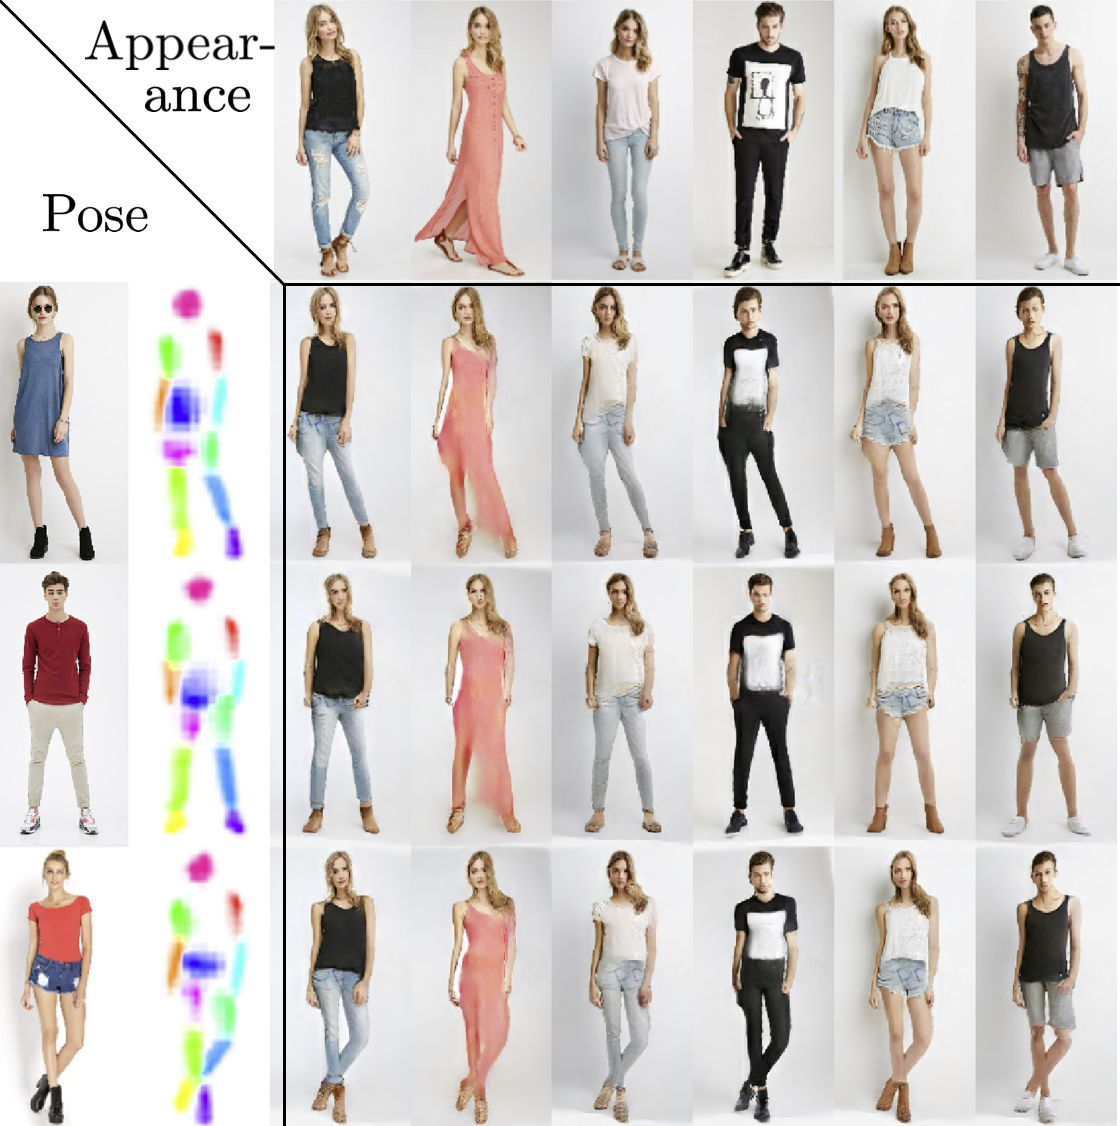
\includegraphics[trim={0cm 0cm 0cm 0cm},clip, width=1.\linewidth]{fig/swappy}
		\caption{Transferring shape and appearance on Deep Fashion. Without annotation the model estimates shape, 2nd column. Target appearance is extracted from images in top row to synthesize images. Note that we trained without image pairs only using synthetic transformations.
		%for training we had no image pairs but only synthetic transformations.
		%without being explicitly trained for this task.
		All images are from test set.}
		\label{fig:allswaps}
	\end{figure}
	\begin{table}
	\caption{Mean average precision (mAP) and rank-n accuracy for person re-identification on synthesized images after performing shape/appearance swap. Input images from Deep Fashion test set. Note \cite{Esser:2018ue} is supervised w.r.t. shape.}
	\label{tab:reid}
	\begin{tabular}{l|cccr}
		\hline
		& mAP & rank-1 & rank-5 & rank-10 \\ \hline
		VU-Net \cite{Esser:2018ue} & 88.7\% & 87.5\% & {98.7}\% & {99.5}\% \\
		Ours & {90.3}\% & {89.4}\% &{98.2}\% & {99.2}\% \\ \hline
	\end{tabular}
\end{table}
\begin{table}
	\caption{Percentage of Correct Keypoints (PCK) for pose estimation on shape/appearance swapped generations.\;$\alpha$ is pixel distance divided by image diagonal. Note that \cite{Esser:2018ue} serves as upper bound, as it uses the groundtruth shape estimates.}
	%shape supervision.}
	\label{tab:pose}
	\begin{tabular}{l|cccr}
		\hline
		$\alpha$ & $2.5\%$ &  $5\%$ & $7.5\%$ & $10\%$ \\ \hline
		VU-Net \cite{Esser:2018ue} & {95.2}\% & {98.4}\% & {98.9}\% & {99.1}\% \\
		Ours & 85.6\% & 94.2\% &96.5\% & 97.4\% \\ \hline
	\end{tabular}
\end{table}
% BBC THUMB
%
\begin{figure}[t]
	\centering
	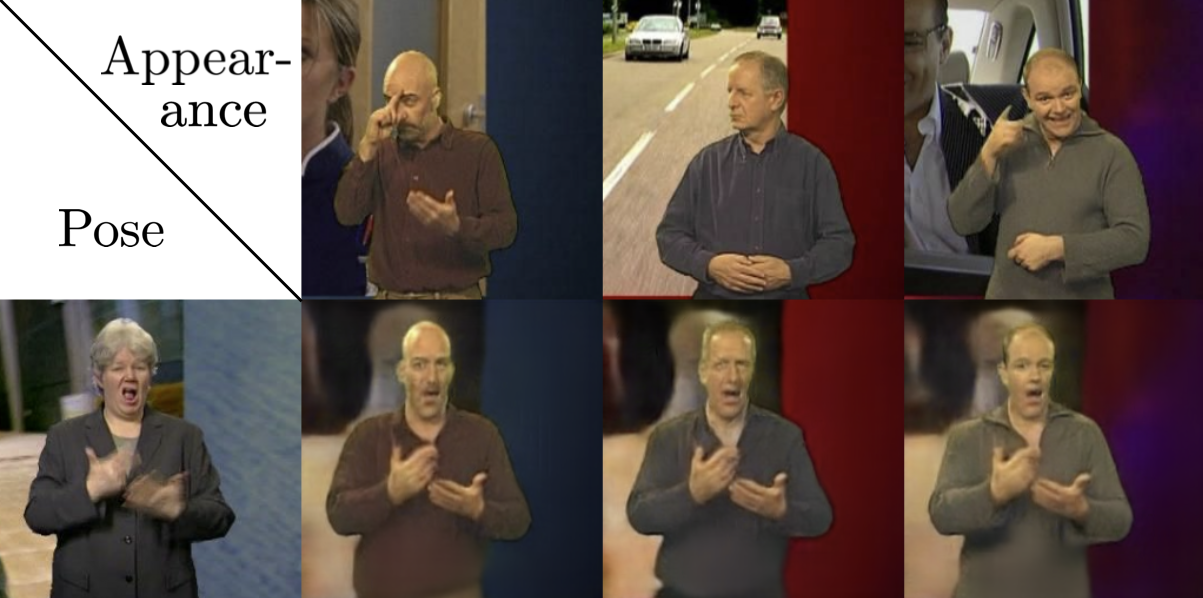
\includegraphics[trim={0cm 0cm 0cm 0cm},clip, width=1.\linewidth]{fig/bbcthumb}
	\caption{Video-to-video translation on BBC Pose. Top-row: target appearances, left: target pose.
	%The target appearances are from the train set, while the target pose is from the test set.
	Note that even fine details in shape are accurately captured. See supplementary for videos.}
	\label{fig:bbcthumb}
\end{figure}

	Disentangled representations of object shape and appearance allow to alter both properties individually to synthesize new images. The ability to flexibly control the generator allows, for instance, to change the pose of a person or their clothing. In contrast to previous work \cite{esser18, denton17disvideo, ma17poseguided, ma17disperson, debem18dgpose, jakab18},
	we achieve this ability without requiring supervision \textit{and} using a flexible part-based model instead of a holistic representation. This allows to explicitly control the parts of an object that are to be altered. We quantitatively compare against \emph{supervised} state-of-the-art disentangled synthesis of human figures. Also we qualitatively evaluate our model on unsupervised synthesis of still images, video-to-video translation, and local editing for appearance transfer.


	t-SNE of Shape Representation
	t-SNE of Appearance Representation


	\subsection{Disentangling Pose and Appearance}


	On Deep Fashion \cite{liu16deepfashion, liu16deepfashionwild}, a benchmark dataset for supervised disentangling methods, the task is to separate person ID (appearance) from body pose (shape) and then synthesize new images for previously unseen persons from the test set in eight different poses. We randomly sample the target pose and appearance conditioning from the test set. Fig. \ref{fig:allswaps} shows qualitative results.
	We quantitatively compare against supervised state-of-the-art disentangling \cite{esser18} by evaluating \emph{i)} invariance of appearance against variation in shape by the re-identification error and \emph{ii)} invariance of shape against variation in appearance by the distance in pose between generated and pose target image.

	\subsubsection{ReID}
	t-SNE of IDs
	Own, Other (stronger statement)
	To evaluate appearance we fine-tune an ImageNet-pretrained \cite{russakovsky15imagenet} Inception-Net \cite{szegedy15inception} with a re-identification (ReID) algorithm \cite{xiao17reidjoint} via a triplet loss \cite{hermans17reidtriplet} to the Deep Fashion training set.
	On the generated images we evaluate the standard metrics for ReID, mean average precision (mAP) and rank-1, -5, and -10 accuracy in Tab. \ref{tab:reid}.
	Although our approach is unsupervised it is competitive compared to the supervised VU-Net \cite{esser18}.



	\subsubsection{Pose}
	To evaluate shape, we extract keypoints using the pose estimator \cite{cao17affinityfield}. Tab. \ref{tab:pose} reports the difference between generated and pose target in percentage of correct keypoints (PCK). As would be expected, VU-Net performs better, since it is trained with exactly the keypoints of \cite{cao17affinityfield}. Still our approach achieves an impressive PCK without supervision underlining the disentanglement of appearance and shape.


	PCK Curve
	\subsection{Factorizing into Parts}
	% PART SWAPS
	\begin{figure}[t]
		\begin{subfigure}{0.49\linewidth}
		\centering
		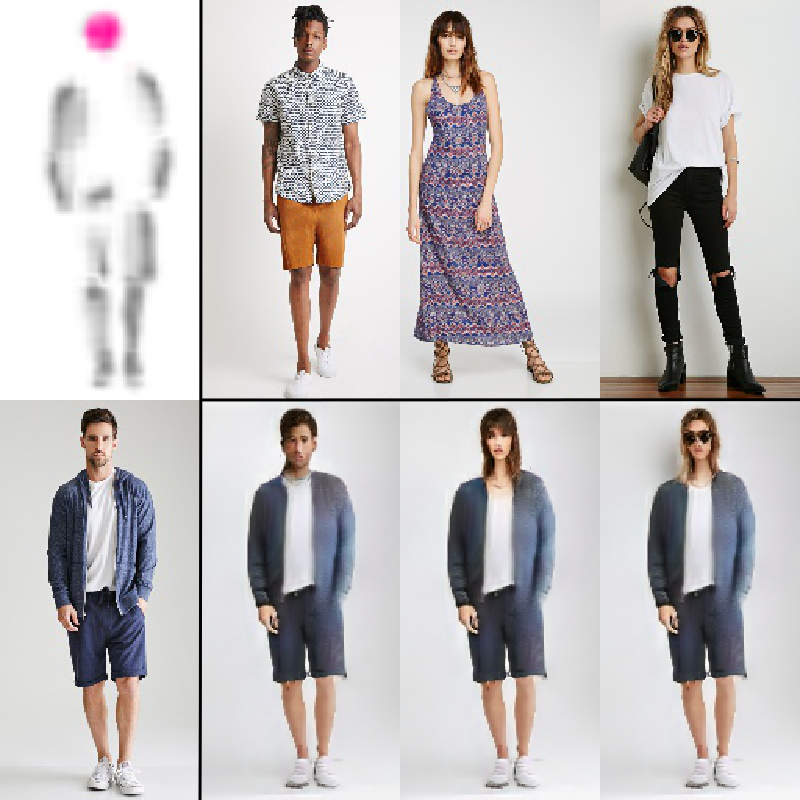
\includegraphics[trim={0cm 0cm 0cm 0cm},clip, width=1.\linewidth]{fig/part_head}\caption{}
		\label{fig:part3_00}
		\end{subfigure}
		\begin{subfigure}{0.49\linewidth}
		\centering
		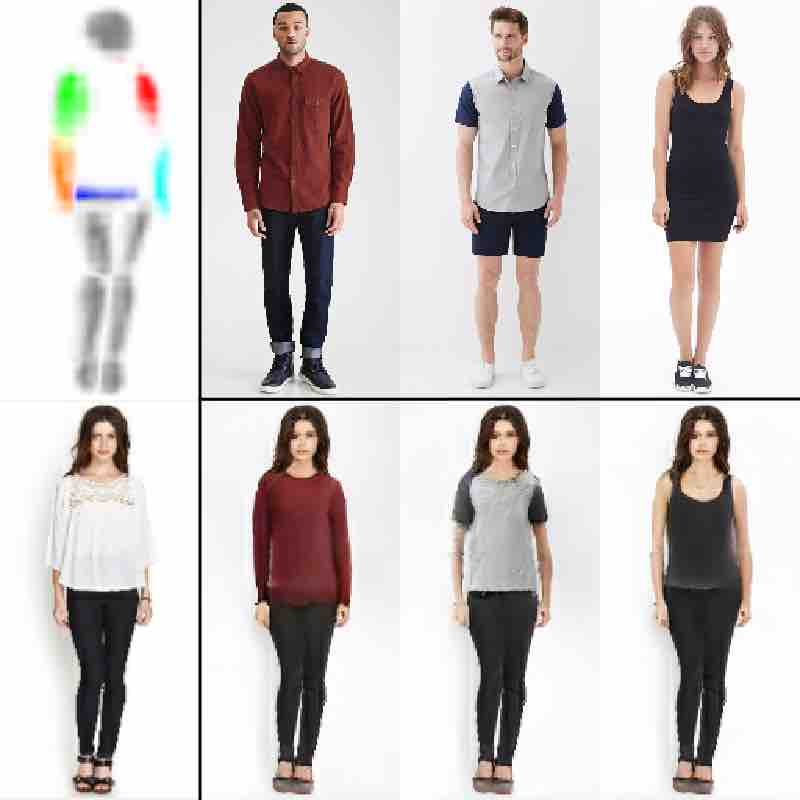
\includegraphics[trim={0cm 0cm 0cm 0cm},clip, width=1.\linewidth]{fig/part_body}\caption{}
		\label{fig:part3_11}
		\end{subfigure}
		\begin{subfigure}{0.49\linewidth}
		\centering
		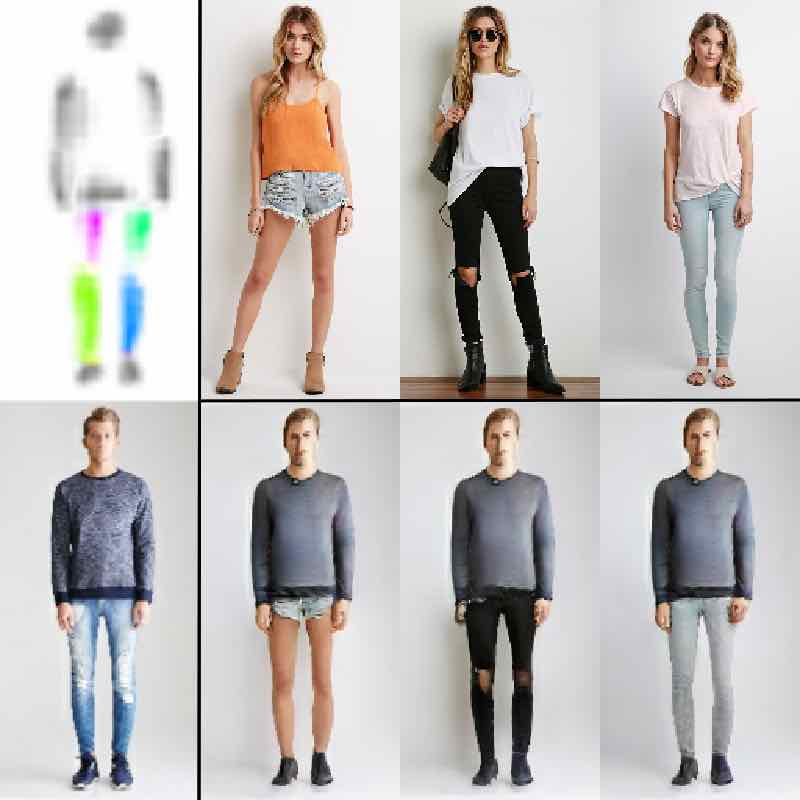
\includegraphics[trim={0cm 0cm 0cm 0cm},clip, width=1.\linewidth]{fig/part_legs}\caption{}
		\label{fig:part3_21}
		\end{subfigure}
		\begin{subfigure}{0.49\linewidth}
		\centering
		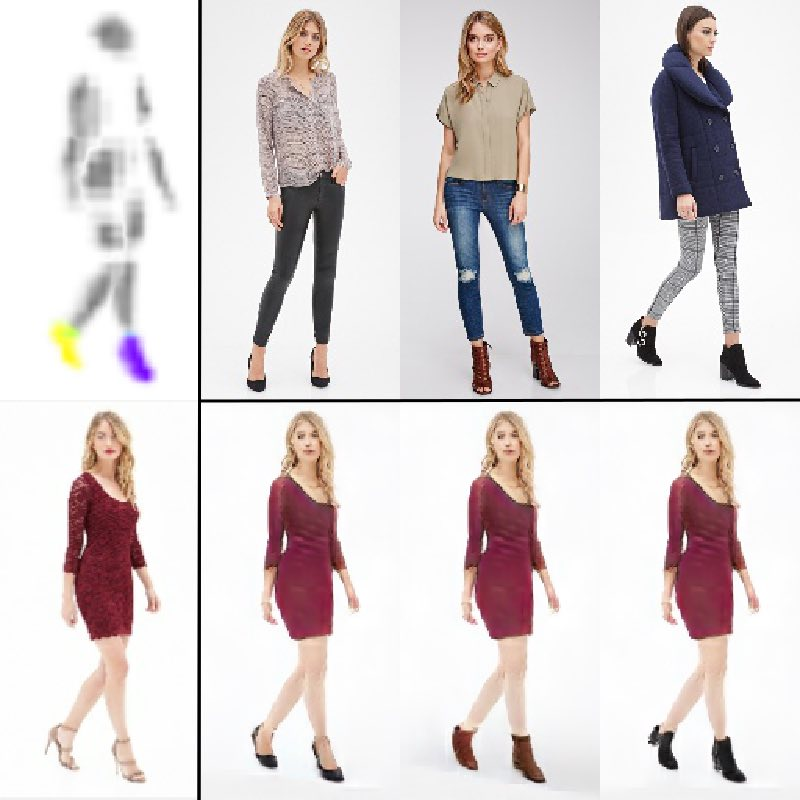
\includegraphics[trim={0cm 0cm 0cm 0cm},clip, width=1.\linewidth]{fig/part_shoe}\caption{}
		\label{fig:part3_30}
		\end{subfigure}
		\caption{Swapping part appearance on Deep Fashion. Appearances can be exchanged for parts individually and without altering shape. We show part-wise swaps for (a) head (b) torso (c) legs, (d) shoes. All images are from the test set.}
		\label{fig:partswaps}
	\end{figure}
		Own Dataset: Move KP
		DeepFashion: exchange parts
\section{Follow-Up}
	\begin{itemize}
		\item make generative:(KP distribution estimation, variational features).
		\item make video generation possible (RNN on KP vector).
		\item better transformations -> appearance locally (around parts changed), appearance changed perceptually -> style transfer
	\end{itemize}





